\documentclass[aps,prd,twocolumn,superscriptaddress,nofootinbib,longbibliography]{revtex4-2}

\usepackage[utf8]{inputenc}
\usepackage[T1]{fontenc}
\usepackage{amsmath,amssymb,bm}
\usepackage{mathrsfs}
\usepackage{graphicx}
\usepackage{booktabs}
\usepackage{array}
\usepackage[colorlinks=true,linkcolor=blue,citecolor=blue,urlcolor=blue]{hyperref}

\newcommand{\dd}{\mathrm{d}}
\newcommand{\Lag}{\mathcal{L}}
\newcommand{\LD}{\mathfrak{L}}
\newcommand{\calS}{\mathcal{S}}
\newcommand{\calC}{\mathcal{C}}
\newcommand{\calD}{\mathcal{D}}
\newcommand{\Mp}{M_{\rm p}}
\newcommand{\Lam}{\Lambda}
\newcommand{\LCDM}{\Lambda{\rm CDM}}
\newcommand{\DES}{\mathrm{DES}}
\newcommand{\DESI}{\mathrm{DESI}}
\newcommand{\SN}{\mathrm{SN}}
\newcommand{\BAO}{\mathrm{BAO}}
\newcommand{\varphione}{\varphi_1}
\newcommand{\varphitwo}{\varphi_2}
\newcommand{\chiT}{\chi^2_{\rm tot}}
\newcommand{\Riemsq}{R_{\mu\nu\rho\sigma}R^{\mu\nu\rho\sigma}}

\begin{document}

\preprint{AI-MG-v5.2.2-agent}

\title{Dark Energy Autonomous Search from Cosmological Background Data}

\author{Cooper Niu}
\affiliation{Department of Physics, Brown University, Providence, Rhode Island 02912, USA}

\author{Wenrong Sun}
\affiliation{Department of Physics, Brown University, Providence, Rhode Island 02912, USA}

\date{\today}


\begin{abstract}
We present a physics-first autonomous search for two-scalar modified-gravity backgrounds and use it to benchmark large-language-model proposal policies under an identical deterministic validation pipeline. Candidate theories are generated as covariant, dimension-balanced Lagrangian densities built from curvature tensors, covariant derivatives, and two scalar fields. They are then subjected to symbolic FLRW equation-of-motion filtering, algebraic cancellation of independent third- and higher-time derivatives, Builder conversion into numerical models, and direct comparison with DES type-Ia supernovae and DESI Data Release 2 baryon-acoustic-oscillation distances. The AI component affects only the proposal distribution over legal operator combinations and explicit parameter samples; ghost filtering, numerical regularity, constraint preservation, and the final ranking by $\chi^2_{\rm tot}$ are determined by the physics code. The unified benchmark uses five agents: GPT-5.5, Claude Opus 4.8, Gemini 3.1 Pro, Qwen 3.7 Plus, and DeepSeek V4 Pro. Qwen obtains the best open-search value, $\chi^2_{\rm tot}=1637.930$, while DeepSeek obtains the strongest non-EH branch, $\chi^2_{\rm tot}=1693.860$. The fixed $\Lambda$CDM reference gives $\chi^2_{\rm tot}=1645.28$, so all agents locate competitive Einstein--Hilbert-anchored backgrounds, whereas genuinely non-EH backgrounds remain substantially less favored. These results benchmark proposal policies for background discovery; they do not by themselves establish full covariant ghost freedom, perturbation stability, structure-growth viability, gravitational-wave consistency, or local-gravity screening.
\end{abstract}

\maketitle


\section{Introduction}
\label{sec:introduction}

The observed acceleration of the Universe is one of the clearest indications that either the cosmic energy budget or the gravitational sector is not yet fully understood.  The minimal $\Lambda$CDM model gives a compact effective description of current background data, but it treats the late-time vacuum-energy scale as an input and does not explain whether the acceleration is produced by a rigid cosmological constant, additional fields, or modified gravitational dynamics.  Scalar-tensor and higher-curvature theories offer a controlled language for testing this possibility, but they also create a search problem: once curvature invariants, covariant derivatives, and multiple scalar fields are allowed, the space of covariant Lagrangians is far too large to inspect manually \cite{Clifton2012,SotiriouFaraoni2010,Horndeski1974}.

Most points in this large theory space are not physically acceptable.  Generic higher-derivative theories contain Ostrogradsky modes \cite{Ostrogradsky1850}; many proposed covariant densities do not admit a regular FLRW initial-value problem; many numerically regular branches violate the modified Friedmann constraint during integration; and most surviving backgrounds fit DES supernova and DESI BAO distances poorly.  A useful autonomous search must therefore be physics-first: an agent may propose structures, but deterministic symbolic and numerical code must decide whether the proposal is legal, stable at the background-filter level, numerically solvable, and empirically competitive.

The framework used here follows this division of labor.  A proposal model chooses a scalar configuration, a grammar-constrained set of covariant operators, and an explicit list of parameter samples.  The proposal is then compiled into an isolated Lagrangian and passed through the same pipeline for every agent: symbolic FLRW variation, equation-level cancellation of independent third- and higher-time derivatives, Builder construction of a dimensionless initial-value problem, Solver integration, modified Friedmann-constraint monitoring, and comparison with DES-SN and DESI-DR2 BAO data \cite{DES2024SN,DESI2025BAO}.  The AI system does not estimate $\chi^2$, bypass the grammar, or override a failed physics stage.  This design is close in spirit to formal-language approaches to autonomous theory discovery, but the grammar and validation stages are those of modified gravity rather than particle interactions \cite{Alexander2026Albert}.

The present paper has two goals.  First, it summarizes the covariant theory space, FLRW derivative-order filter, constraint logic, dimensionless cosmological system, and sampling prescription used in the current code base.  These ingredients define what is meant by an accepted background branch.  Second, it reports a matched five-model benchmark of the proposal layer.  We compare GPT-5.5, Claude Opus 4.8, Gemini 3.1 Pro, Qwen 3.7 Plus, and DeepSeek V4 Pro on the same cold-start task, with two discovery sectors: an open-search sector that may include the Einstein--Hilbert anchor, and a non-EH sector that forbids the bare $R$ term and searches for new-physics backgrounds without explicit EH support.  The comparison is organized around global optimum quality, new-physics discovery, speed/efficiency, robustness/stability, and acceptance rate.

The results should be interpreted with care.  The background data strongly favor EH-anchored scalar histories, and many low-$\chi^2$ operator lists are nearly degenerate with simple EH plus scalar baselines on FLRW.  Conversely, the non-EH sector repeatedly finds a recognizable $\phi_2$ curvature-coupled branch near $\chi^2_{\rm tot}\simeq 1946.87$, but this branch is not competitive with the open-search optimum.  These outcomes are useful: they identify where the current grammar and priors easily reproduce high-quality expansion histories, where genuinely non-EH searches remain difficult, and how different proposal models trade exploitation, exploration, and wall-clock speed.  They are not final claims of full theory viability; perturbation stability, structure growth, gravitational waves, local tests, and a more complete operator-redundancy audit remain separate validation layers.

\section{Covariant Theory Space}
\label{sec:theory-space}

\subsection{Dimension-balanced effective Lagrangians}
\label{subsec:dimension-balanced}

We consider a broad EFT-like space of metric theories containing two scalar fields, $\phi_1$ and $\phi_2$, with different characteristic scales.  A generated theory is stored and validated as a Lagrangian density,
\begin{equation}
\calS=\int \dd^4x\,\mathscr{L},
\qquad
\mathscr{L}=\sqrt{-g}\,\Lag ,
\label{eq:action}
\end{equation}
with the scalar bracket
\begin{equation}
\Lag=
\Mp^2\sum_{I\in G\cup N}
c_I\Lam^{2-d_I}O_I
+
\sum_{J\in S}c_J\Lam^{4-d_J}S_J
+
\Lag_{\rm fixed}.
\label{eq:lagrangian}
\end{equation}
Here $G$ denotes pure-curvature invariants, $N$ non-minimal scalar-curvature invariants, and $S$ pure-scalar generated invariants.  The integer $d_I$ is the mass dimension of the corresponding covariant scalar.  The factors of $\Mp^2$ and $\Lam$ ensure that each term in the density $\mathscr{L}$ has the correct mass dimension.  Thus a candidate is not specified by an operator label alone; its sector, coefficient, cutoff power, Planck-mass prefactor, fixed scalar matter terms, and outer $\sqrt{-g}$ are part of the physical theory.

The candidate building blocks include
\begin{equation}
R,\qquad R_{\mu\nu},\qquad R^\rho{}_{\sigma\mu\nu},\qquad
\nabla_\mu,\qquad \phi_1,\qquad \phi_2 .
\end{equation}
Examples of generated invariants are
\begin{equation}
R^2,\qquad
R_{\mu\nu}R^{\mu\nu},\qquad
\phi_1^2R,\qquad
\nabla_\mu\phi_1\nabla_\nu\phi_1R^{\mu\nu},\qquad
\Box\phi_1\,R.
\end{equation}
Up to mass dimension six, there are 141 independent curvature invariants on the FLRW background.
The scalar configurations are 
\begin{equation}
\hbox{none},\qquad \phi_1\hbox{ only},\qquad \phi_2\hbox{ only},\qquad \phi_1\text{ and }\phi_2 .
\end{equation}
When a scalar is active, the fixed matter sector contains a canonical kinetic term and either a quadratic or an axion-like potential:
\begin{align}
\Lag_{\rm fixed}^{(i)}
&=-\frac12 g^{\mu\nu}\nabla_\mu\phi_i\nabla_\nu\phi_i - V_i(\phi_i),\\
V_i(\phi_i)
&=\frac12 m_i^2\phi_i^2
\quad{\rm or}\quad
m_i^2f_i^2\left[1-\cos\left(\frac{\phi_i}{f_i}\right)\right].
\label{eq:fixed-sector}
\end{align}


The two scalar fields play different roles in the current theory grammar.  The first scalar is naturally measured in Planck units,
\begin{equation}
\phi_1=\Mp\varphione,
\end{equation}
while the second is measured in cutoff units,
\begin{equation}
\phi_2=\Lam\varphitwo .
\end{equation}
This hierarchy allows the search to include both Planck-normalized scalar-tensor sectors and cutoff-normalized EFT scalar structures.  The distinction matters because a term such as $\phi_2 R$ carries a different scale from $\phi_1 R$, even when their dimensionless field amplitudes are comparable.  It is therefore useful to parameterize the EFT cutoff in units of the present Hubble scale,
\begin{equation}
\lambda_H\equiv\frac{\Lam}{H_0}.
\label{eq:lambdaH}
\end{equation}
With $h\equiv H/H_0$, the dimensionless ratio between the background expansion scale and the cutoff is simply $H/\Lam=h/\lambda_H$.  This quantity enters the validation-stage scale-separation cut introduced in Sec.~\ref{sec:ivp}.

\section{Mini-Superspace and Background Physical Filtering}
\label{sec:ghost}

\subsection{Background equations}
\label{subsec:background-eom}

The first physical filter is applied after reducing the covariant theory on the spatially flat FLRW metric
\begin{equation}
\dd s^2=-N(t)^2\dd t^2+a(t)^2\delta_{ij}\dd x^i\dd x^j .
\label{eq:flrw}
\end{equation}
The minisuperspace variation gives
\begin{equation}
\delta S=\int \dd t\left(E_N\delta N+E_a\delta a+\sum_iE_{\phi_i}\delta\phi_i\right),
\label{eq:variation}
\end{equation}
where the inactive scalar equations are omitted.  After variation, the equations are evaluated in cosmic-time gauge, $N=1$:
\begin{equation}
E_N=0,\qquad E_a=0,\qquad E_{\phi_i}=0 .
\label{eq:eom-set}
\end{equation}
The lapse equation is not discarded.  It is the modified Friedmann equation, while $E_a$ and $E_{\phi_i}$ determine the dynamical evolution.


\subsection{Ostrogradsky ghost and FLRW cancellation relations}
\label{subsec:ostro}

Higher-curvature and derivative scalar-curvature operators generically produce equations containing third or higher time derivatives of $a(t)$ and $\phi_i(t)$.  If such derivatives represent independent initial data, the theory contains an Ostrogradsky mode: the Hamiltonian is unbounded and the background branch is a physically unacceptable ghost\cite{Ostrogradsky1850}.  The pipeline therefore treats the derivative order of the FLRW equations as a hard physical constraint before any likelihood evaluation.

The raw proposal grammar is deliberately broader than the standard Horndeski basis.  It can contain operators such as $R^2$, $R^3$, $\nabla R\nabla R$, or mixed scalar-curvature contractions.  These monomials should not be read as arbitrary higher-derivative theories after acceptance.  The EOM stage first derives the gauge-fixed FLRW equations and expands their forbidden higher-derivative part schematically as
\begin{equation}
E_A=E_A^{\leq 2}+
\sum_{B}\sum_{r\geq 3}{\cal A}_{AB}^{(r)}(a,\dot a,\phi_i,\dot\phi_i;c_I)
\,y_B^{(r)},
\label{eq:forbidden-derivatives}
\end{equation}
where $A$ labels the lapse, scale-factor, and active-scalar equations, $y_B\in\{a,\phi_i\}$, and the ${\cal A}_{AB}^{(r)}$ are algebraic functions of the operator coefficients and lower-derivative variables.  The background cancellation filter solves the coefficient constraints
\begin{equation}
{\cal A}_{AB}^{(r)}=0
\qquad
\hbox{for all independent }B\hbox{ and }r\geq 3,
\label{eq:cancellation-relations}
\end{equation}
and substitutes the resulting branch relations before passing the model to the Builder and Solver.  A model may therefore contain a displayed $R^2$, $R^3$, or derivative-curvature operator only as part of a coefficient-restricted FLRW-degenerate combination.  If the required relations force the relevant correction to zero, the model is interpreted as the corresponding lower-complexity branch rather than as evidence for an active higher-curvature correction.

This condition is Horndeski/DHOST-like in spirit, because it removes the would-be Ostrogradsky data by degeneracy rather than by assuming small higher derivatives \cite{Horndeski1974,Langlois2016DHOST}.  It is not identical to imposing the full covariant Horndeski Lagrangian at the proposal stage.  The proposal space is broader, while the acceptance condition is narrower and equation-level: the accepted branch must have FLRW equations with no independent third- or higher-time derivatives after the coefficient relations are imposed.

\subsection{The modified Friedmann constraint}
\label{sec:hamiltonian}
\label{subsec:modified-friedmann}



In ordinary GR, the FLRW lapse $N$ appears without time derivatives after the Einstein--Hilbert boundary term is handled.  The momentum conjugate to $N$ vanishes, and preserving this primary constraint gives the Hamiltonian constraint, which reduces to the Friedmann equation.  In a raw modified-gravity minisuperspace Lagrangian, however, $N$ may appear with derivatives before integrations by parts or before imposing the background derivative-cancellation relations.  Therefore the simple GR statement ``the lapse is a Lagrange multiplier'' is not always the cleanest way to identify the constraint.

The more robust argument comes from residual time-reparametrization invariance.  Under
\begin{equation}
t\rightarrow t-\xi(t),
\end{equation}
the minisuperspace variables transform as
\begin{equation}
\delta_\xi a=\xi\dot a,\qquad
\delta_\xi\phi_i=\xi\dot\phi_i,\qquad
\delta_\xi N=(N\xi)^{\cdot}.
\label{eq:time-diffeo}
\end{equation}
Invariance of the action under this transformation gives the off-shell Noether identity
\begin{equation}
N\dot E_N-\dot a\,E_a-\sum_i\dot\phi_i\,E_{\phi_i}=0.
\label{eq:noether}
\end{equation}
This is the minisuperspace form of the Bianchi identity.  It holds before imposing the equations of motion.



After gauge fixing to $N=1$, Eq.~\eqref{eq:noether} becomes
\begin{equation}
\dot E_N=\dot a\,E_a+\sum_i\dot\phi_i\,E_{\phi_i}.
\label{eq:noether-gauge}
\end{equation}
Suppose the background derivative-cancellation relations have made the dynamical equations $E_a=0$ and $E_{\phi_i}=0$ at most second order in time derivatives.  Then the right-hand side of Eq.~\eqref{eq:noether-gauge} contains no independent third derivatives.

If the gauge-fixed lapse equation $E_N|_{N=1}$ contained an acceleration, schematically
\begin{equation}
E_N|_{N=1}=C(a,\dot a,\ddot a,\phi_i,\dot\phi_i,\ddot\phi_i),
\end{equation}
then its time derivative would contain independent third derivatives:
\begin{equation}
\dot E_N|_{N=1}
\supset
\frac{\partial C}{\partial \ddot a}a^{(3)}
+\sum_i
\frac{\partial C}{\partial \ddot\phi_i}\phi_i^{(3)}.
\end{equation}
These terms cannot be matched by the right-hand side of Eq.~\eqref{eq:noether-gauge}.  Since the identity is off shell and holds for arbitrary field profiles, the coefficients of all independent third derivatives must vanish.  Therefore
\begin{equation}
E_N|_{N=1}=C_N(a,\dot a,\phi_i,\dot\phi_i),
\label{eq:first-order-constraint}
\end{equation}
and the lapse equation is a first-order constraint on FLRW initial data, not an independent second-order dynamical equation.


The same identity guarantees propagation of the constraint.  On solutions of the dynamical equations,
\begin{equation}
E_a=0,\qquad E_{\phi_i}=0,
\end{equation}
Eq.~\eqref{eq:noether-gauge} implies
\begin{equation}
\dot E_N=0.
\end{equation}
Thus if the initial data satisfy
\begin{equation}
E_N(t_0)=0,
\end{equation}
then the background evolution preserves
\begin{equation}
E_N(t)=0.
\end{equation}
This justifies using the lapse equation to solve for one initial velocity and then monitoring the residual constraint throughout numerical integration.

The result is deliberately limited to the background construction: within the FLRW derivative-cancelled sector, the lapse equation is a first-order modified Friedmann constraint, and the dynamical equations preserve it once it is imposed on the initial data.  The wider domain of validity of this minisuperspace statement is summarized next.

\subsection{Scope of the background filter}
\label{subsec:ghost-scope}

The preceding analysis imposes two distinct background-level requirements.  First, Eq.~\eqref{eq:cancellation-relations} removes all independent third- and higher-time derivatives from the gauge-fixed FLRW equations.  Second, the residual time-reparametrization identity makes the lapse equation a preserved first-order constraint on the accepted branch.  Together these conditions are necessary for the background initial-value problem, but they are not a sufficient proof of full covariant ghost freedom.  They do not establish the complete ADM/Dirac constraint algebra, the quadratic action for scalar and tensor perturbations, the sign of the kinetic matrix, gradient stability, the tensor propagation speed, or stability on non-FLRW backgrounds.  These checks are logically separate from the background search.  In this paper, ``accepted'' means that a branch has passed the FLRW derivative-order filter, admits a regular background initial-value problem, preserves the modified Friedmann constraint numerically, satisfies the stated background EFT cut, and yields a finite DES-SN plus DESI-DR2 BAO score.  It does not mean that the theory is already a fully viable modified-gravity model.

On this restricted background sector, the modified Friedmann constraint can be used to select initial data and the remaining equations can be cast as the dimensionless first-order system constructed next.

\section{Dimensionless Cosmological Initial-Value Problem}
\label{sec:ivp}

The numerical evolution uses e-fold time
\begin{equation}
x=\ln a=-\ln(1+z),
\qquad
h=\frac{H}{H_0},
\label{eq:xh}
\end{equation}
so that
\begin{equation}
\frac{\dd}{\dd t}=H_0h\frac{\dd}{\dd x}.
\label{eq:chain-rule}
\end{equation}
The relevant substitutions include
\begin{align}
\dot a&=H_0e^xh,
&
\ddot a&=H_0^2e^x(h^2+hh_x),\\
\dot\phi_1&=\Mp H_0h q_1,
&
\ddot\phi_1&=\Mp H_0^2h(h_xq_1+hq_{1x}),\\
\dot\phi_2&=H_0^2\lambda_H h q_2,
&
\ddot\phi_2&=H_0^3\lambda_H h(h_xq_2+hq_{2x}),
\label{eq:rescalings}
\end{align}
where
\begin{equation}
q_i=\frac{\dd\varphi_i}{\dd x}.
\end{equation}
Masses and decay constants are written as
\begin{equation}
m_1=H_0\mu_1,\qquad
m_2=\Lam\mu_2,\qquad
f_1=\Mp \bar f_1,\qquad
f_2=\Lam \bar f_2 .
\end{equation}

After these substitutions, the Builder forms dimensionless equations
\begin{equation}
C_N=0,\qquad C_a=0,\qquad C_{\phi_i}=0.
\end{equation}
The constraint $C_N=0$ is imposed at $x=0$ with $h(0)=1$.  The dynamical equations are solved algebraically for the highest e-fold derivatives,
\begin{equation}
\bm u=(h_x,q_{1x},q_{2x})^T.
\end{equation}
When a regular branch exists, the result is an explicit first-order system,
\begin{equation}
\frac{\dd}{\dd x}
\begin{pmatrix}
h\\ \varphione\\ q_1\\ \varphitwo\\ q_2
\end{pmatrix}
=
\begin{pmatrix}
F_h\\ q_1\\ F_1\\ q_2\\ F_2
\end{pmatrix},
\label{eq:first-order}
\end{equation}
with absent scalar variables omitted.  The trajectory is rejected if the constraint drifts beyond the production tolerance,
\begin{equation}
\max_x|C_N(x)|>10^{-4}.
\label{eq:constraint-cut}
\end{equation}
It is also rejected if the background expansion scale approaches the cutoff.  The validation-stage scale-separation cut is
\begin{equation}
\epsilon_H\equiv
\max_x\frac{|H(x)|}{\Lam}
=
\max_x\frac{|h(x)|}{\lambda_H}
<0.1 .
\label{eq:eft-cut}
\end{equation}
This is a hard background-level rejection criterion.  It ensures that the accepted trajectory remains below the cutoff scale probed by the homogeneous expansion, but it should not be read as a complete proof that the full EFT expansion is controlled.  The stronger field-excursion, kinetic, and operator-hierarchy diagnostics are discussed in Sec.~\ref{sec:validation-boundaries}.

\section{Cosmological Observables}
\label{sec:observables}

Each accepted solution gives a Hubble history $H(z)=H_0h(z)$.  The supernova distance modulus is computed from
\begin{equation}
D_L(z)=(1+z_{\rm hel})\frac{c}{H_0}
\int_0^{z_{\rm HD}}\frac{\dd z'}{h(z')},
\label{eq:luminosity-distance}
\end{equation}
with an analytically profiled absolute-magnitude offset.  The supernova likelihood therefore mainly constrains the relative shape of the distance-redshift relation.

The BAO observables are computed from the same background solution:
\begin{align}
\calD_M(z)&=\int_0^z\frac{\dd z'}{h(z')},\\
\calD_H(z)&=\frac{1}{h(z)},\\
\calD_V(z)&=\left[\frac{z\calD_M(z)^2}{h(z)}\right]^{1/3}.
\label{eq:bao}
\end{align}
In this background-only analysis, the BAO scale is profiled as a nuisance parameter.  Thus the DESI comparison should be interpreted as a relative-distance test of the late-time expansion history, not as a complete early-universe calculation of the sound horizon in each modified-gravity theory.

The primary score is
\begin{equation}
\chiT=\chi^2_{\DES\text{-}\SN}+\chi^2_{\DESI\text{-DR2}\,\BAO}.
\label{eq:chi2}
\end{equation}
Models are ranked by $\chiT$, with information criteria recorded only as secondary diagnostics \cite{Akaike1974,Schwarz1978}.


\section{Autonomous Search Strategy}
\label{sec:search}

The autonomous component is an outer loop around the deterministic physics pipeline.  Each proposal is a concrete theory JSON plus an explicit list of numerical parameter samples.  The harness compiles the proposal into an isolated Lagrangian file, runs the EOM and Builder stages, evaluates the supplied samples with the Solver, and writes one factual attempt record.  The proposal model then updates only from current-loop memory: failure tags, accepted-sample rows, $\chi^2$ values, scalar-family statistics, and parameter priors inferred from the same run.  Historical Solver winners are not used as cold-start proposal memory.

The final benchmark uses two proposal sectors.  The open-search sector samples the full grammar and may include the Einstein--Hilbert anchor.  The non-EH sector forbids the bare $R$ anchor and therefore searches for backgrounds whose gravitational dynamics must be supplied by curvature-squared, higher-curvature, derivative-curvature, or scalar-curvature structures.  The target initial proposal budget is split equally,
\begin{equation}
N_{\rm open}:N_{\rm non\text{-}EH}=1:1 .
\label{eq:final-sector-budget}
\end{equation}
Expanded and refined validations do not count toward this initial-theory target; they are repeat evaluations of a promising already-proposed family with larger parameter budgets.

\subsection{Proposal parameters and scan ranges}
\label{subsec:parameter-priors}

Table~\ref{tab:parameter-priors} summarizes the default cold-start ranges for the continuous component of the search.  They are exploration priors rather than physical acceptance conditions: a sample drawn from these ranges is still rejected if it fails the modified Friedmann constraint, violates the background EFT cut, produces an irregular trajectory, or admits no acceptable real root for the constrained initial velocity.

\begin{table*}[t]
\centering
\begin{ruledtabular}
\begin{tabular}{lllll}
Parameter & Dimensionless definition & Applies to & Default range & Sampling scale \\
\hline
$H_0$ & $H_0\,[{\rm km\,s^{-1}\,Mpc^{-1}}]$ & all sectors & $58$--$74$ & linear \\
$\Omega_{m0}$ & $\rho_{m0}/(3\Mp^2H_0^2)$ & all sectors & $0.22$--$0.40$ & linear \\
$\lambda_H$ & $\Lam/H_0$ & all sectors & $5.0\times10^2$--$8.0\times10^4$ & log \\
$\varphi_{1,0}$ & $\phi_1(t_0)/\Mp$ & $\phi_1$ sectors & $10^{-3}$--$10^{1}$ & log \\
$\mu_1$ & $m_1/H_0$ & $\phi_1$ sectors & $10^{-2}$--$10^{2}$ & log \\
$\bar f_1$ & $f_1/\Mp$ & $\phi_1$ axion sectors & $10^{-2}$--$10^{2}$ & log \\
$\varphi_{2,0}$ & $\phi_2(t_0)/\Lam$ & $\phi_2$ sectors & $10^{-5}$--$10^{5}$ in $|\varphi_{2,0}|$ & signed log \\
$q_{2,0}$ & $\dd\varphi_2/\dd\ln a|_{0}$ & two-scalar sectors & $10^{-5}$--$10^{5}$ in $|q_{2,0}|$ & signed log \\
$\mu_2$ & $m_2/\Lam$ & $\phi_2$ sectors & $10^{-5}$--$10^{5}$ & log \\
$\bar f_2$ & $f_2/\Lam$ & $\phi_2$ axion sectors & $10^{-5}$--$10^{5}$ & log \\
$c_I$ & non-EH operator coefficients & generated operators & $10^{-10}$--$10^{20}$ in $|c_I|$ & log, both signs \\
\end{tabular}
\end{ruledtabular}
\caption{Default continuous proposal ranges.  These are broad cold-start exploration priors, not physical acceptance cuts.  The Einstein--Hilbert coefficient is not scanned: when the plain $R$ anchor is present it is fixed to $c_R=1/2$.  In one-scalar models the initial scalar velocity is solved from the modified Friedmann constraint rather than independently sampled.  In two-scalar models $q_{2,0}$ is sampled and the constraint solves for the remaining scalar velocity.}
\label{tab:parameter-priors}
\end{table*}

For higher-dimension curvature corrections, a naive coefficient prior can render the correction effectively invisible because of the associated powers of $\Lam$.  The scans therefore record an effective-size diagnostic and, in selected proposal modes, choose coefficient magnitudes that target weak, moderate, or active fractional corrections relative to the Einstein--Hilbert term.  We estimate
\begin{equation}
\Delta_i\simeq
\left|\frac{c_i}{c_{\rm EH}}\right|\lambda_H^{p_i}{\cal F}_i ,
\label{eq:delta-prior}
\end{equation}
where $p_i$ is the net power of $\lambda_H$ inherited from the dimension-balanced operator and ${\cal F}_i$ denotes the relevant dimensionless field factor.  The weak, moderate, and active-probe target intervals are approximately $10^{-6}$--$10^{-4}$, $10^{-4}$--$10^{-2}$, and $10^{-2}$--$10^{2}$, respectively.  The baseline correction mode, which carries a default weight of $0.10$, does not use Eq.~\eqref{eq:delta-prior}; it samples raw signed-log coefficients from the broad prior.  The remaining default weights are weak $0.30$, moderate $0.30$, and active-probe $0.30$.

The continuous sampler uses a 50/50 hybrid proposal policy.  Half of the samples are agent-exact anchor points and half are stochastic learned-prior draws.  Both halves may consult the current-loop joint parameter memory for up to the configured usage fraction, currently $0.80$: exact samples reuse high-reward parameter vectors from the nearest available family level, while stochastic samples jitter around such vectors in log space.  If no useful current-loop evidence exists, both branches fall back to the learned/default priors with an exploration floor.  These prescriptions are search priors only.  The reported ranking remains the real data value of $\chi^2_{\rm tot}$ written by the Solver.

The final benchmark used asynchronous slots.  Each CPU slot validates one proposed theory at a time; when it finishes, it writes to the shared memory and immediately requests a new proposal using the latest memory.  This avoids waiting for an entire wave when a single symbolic or numerical task is slow.  Each initial theory receives 1000 samples.  If an initial pass produces a promising accepted trajectory, the same family can be expanded to 3000 samples.  Open-search families with $\chi^2_{\rm tot}<1638$ can receive a 5000-sample refinement, while non-EH families with $\chi^2_{\rm tot}<2000$ can receive a dedicated 10000-sample refinement because such hits are rare and are evaluated on their own new-physics scale.  Structural failures such as repeated root failure, missing scalar constraints, dominant constraint drift, integration failure, or symbolic timeout do not trigger expansion.

\subsection{Benchmark design and monitoring}
\label{subsec:benchmark-design}

We analyze a unified five-agent benchmark.  GPT-5.5, Claude Opus 4.8, and Gemini 3.1 Pro are taken from the new 1500-target production runs.  The GPT-5.5 job reached the 72-hour wall-time limit after 1396 recorded initial theories, and we keep the censored result as produced rather than completing it with an additional run.  Qwen 3.7 Plus and DeepSeek V4 Pro are taken from the earlier 2000-target production runs, truncated to task ids not exceeding 1500; expanded and refined validations attached to those first 1500 initial tasks are retained.  We treat these five data sets as one benchmark without drawing a run-source distinction in the figures.

All runs use the same grammar cache, proposal schema, sector split, parameter ranges, initial sample budget, expansion/refinement rules, and ranking by $\chi^2_{\rm tot}$.  The $\Lambda$CDM reference for the same DES-SN plus DESI-DR2 BAO likelihood is
\begin{equation}
\chi^2_{\Lambda{\rm CDM}}=1645.28,
\qquad
H_0=70.0~{\rm km\,s^{-1}\,Mpc^{-1}},
\qquad
\Omega_{m0}=0.306 .
\label{eq:lcdm-reference}
\end{equation}
The benchmark axes are global optimum quality, new-physics search performance, speed/efficiency, robustness/stability, and acceptance rate.  LangSmith tracing was enabled only as a monitoring layer; the paper tables and figures are generated from local JSONL and CSV artifacts, which are the reproducible source of truth.


\section{Benchmark Results}
\label{sec:results}

\begin{figure*}[t]
\centering
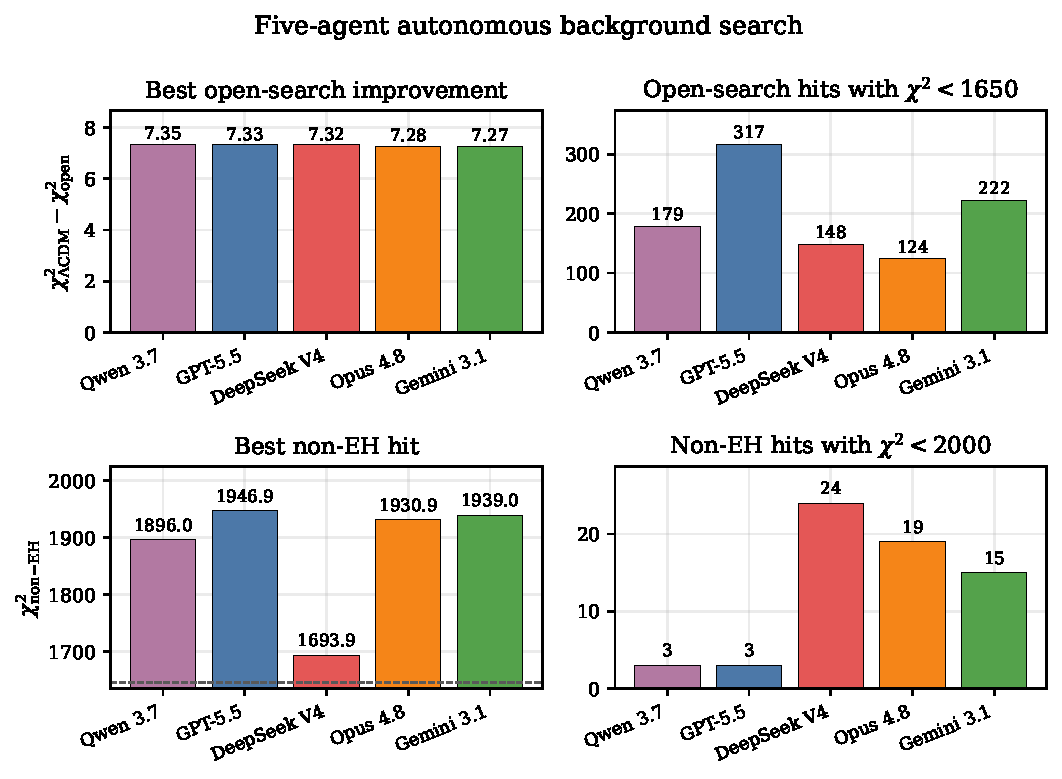
\includegraphics[width=0.88\textwidth]{figures/main_benchmark_dashboard.pdf}
\caption{Unified five-agent benchmark.  The panels show the positive open-search improvement relative to the fixed $\Lambda$CDM reference, the number of high-quality open-search hits, the best non-EH background in the $\chi^2<2000$ display range, and the number of non-EH hits below that threshold.  The dashed reference line in the non-EH best panel is $\Lambda$CDM, while $\chi^2=2000$ is used only as a display and hit-count threshold.}
\label{fig:benchmark-dashboard}
\end{figure*}

\begin{table*}[t]
\centering
\caption{Unified benchmark metrics.  GPT-5.5 is wall-time censored at 1396 recorded initial theories; Qwen 3.7 and DeepSeek V4 use the first 1500 task ids from the earlier 2000-target run.  ``Open'' denotes the full grammar sector, while ``non-EH'' denotes the sector without a bare Einstein--Hilbert $R$ anchor.}
\label{tab:agent-benchmark}
\resizebox{\textwidth}{!}{%
\begin{tabular}{lccccccc}
\toprule
Agent & Initial & Open best & Open median & Open $<1650$ & non-EH best & non-EH $<2000$ & Acc. rate open/non-EH \\
\midrule
Qwen 3.7 & 1500/1500 & 1637.930 & 1639.022 & 179 & 1896.001 & 3 & 0.371 / 0.142 \\
GPT-5.5 & 1396/1500 & 1637.953 & 1638.035 & 317 & 1946.871 & 3 & 0.451 / 0.091 \\
DeepSeek V4 & 1500/1500 & 1637.962 & 1644.949 & 148 & 1693.860 & 24 & 0.352 / 0.164 \\
Opus 4.8 & 1500/1500 & 1638.004 & 3035.050 & 124 & 1930.880 & 19 & 0.343 / 0.165 \\
Gemini 3.1 & 1500/1500 & 1638.012 & 1638.889 & 222 & 1939.014 & 15 & 0.361 / 0.095 \\
\bottomrule
\end{tabular}}
\end{table*}

The open-search sector is highly stable across agents.  Every proposal policy finds an Einstein--Hilbert-anchored basin below the fixed $\Lambda$CDM reference value $\chi^2_{\Lambda{\rm CDM}}=1645.28$.  The best open-search value is obtained by Qwen 3.7, with $\chiT=1637.930$.  The spread among the best open-search values is small, about 0.082 in $\chi^2$, even though the agents differ substantially in accepted medians and hit counts.  This indicates that the background likelihood contains a broad EH-anchored attractor: many operator lists and scalar choices reproduce nearly the same late-time expansion history once the Solver is allowed to scan the explicit parameter samples.

\begin{figure*}[t]
\centering
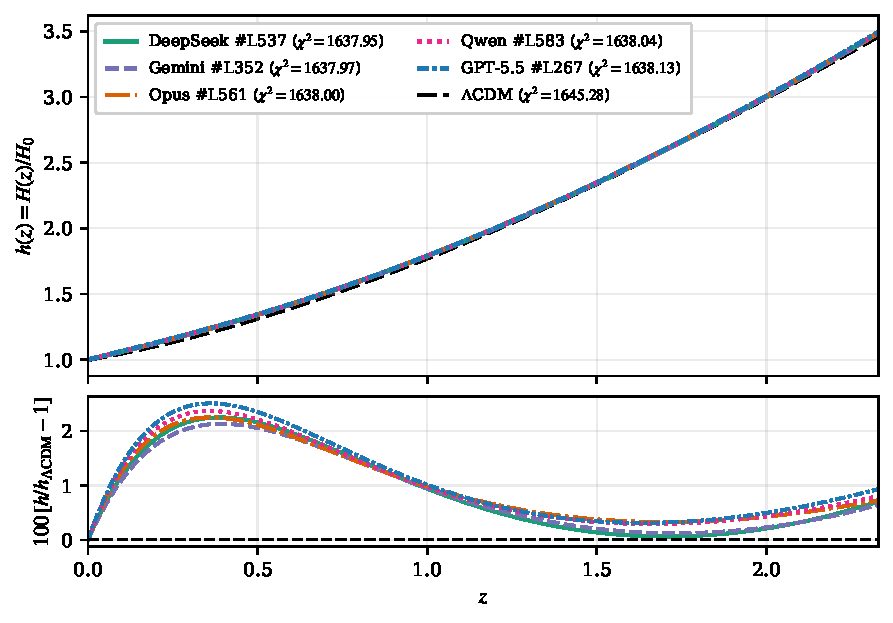
\includegraphics[width=0.88\textwidth]{figures/agent_best_h_lcdm.pdf}
\caption{Replayed best-agent background histories compared with the same fixed $\Lambda$CDM reference used in Eq.~\eqref{eq:lcdm-reference}.  The upper panel shows $h(z)=H(z)/H_0$ for the best representative background from each agent, and the lower panel shows the percent residual relative to $\Lambda$CDM.  This diagnostic uses the dedicated Solver replay curves because the production JSONL pull stores rankings and accepted samples but not every solution-curve CSV.}
\label{fig:agent-best-h-lcdm}
\end{figure*}

\begin{figure*}[t]
\centering
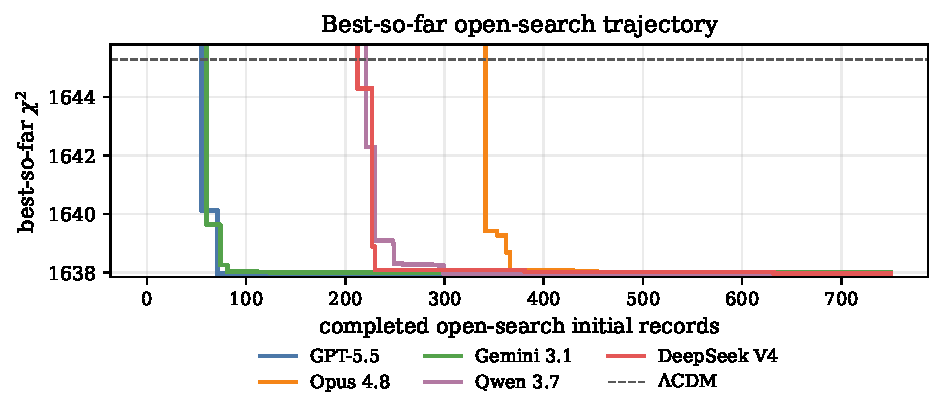
\includegraphics[width=0.88\textwidth]{figures/best_so_far_open_search.pdf}
\caption{Best-so-far open-search value as a function of completed open-search initial records.  The dashed line is the fixed $\Lambda$CDM reference.}
\label{fig:best-so-far-open}
\end{figure*}

\begin{figure*}[t]
\centering
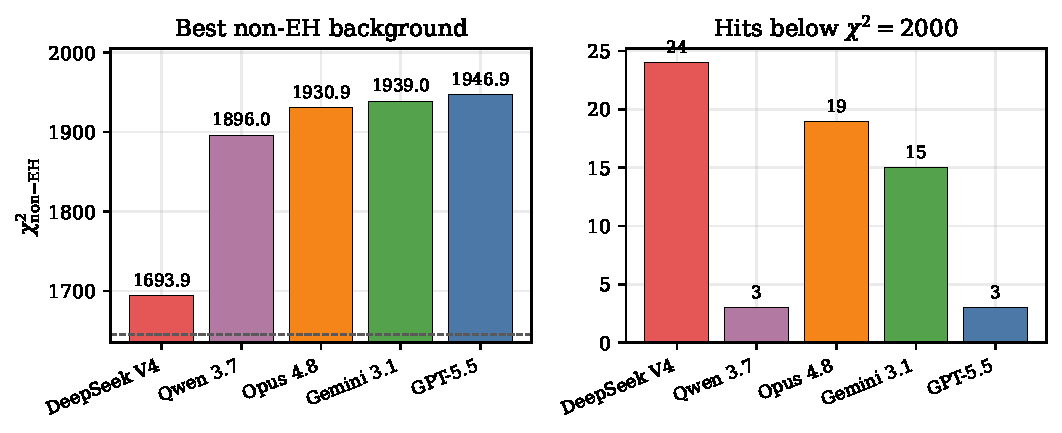
\includegraphics[width=0.88\textwidth]{figures/non_eh_summary.pdf}
\caption{Non-EH search summary.  The left panel shows the best non-EH background found by each agent, restricted to the display range below $\chi^2=2000$; the dashed reference line is the fixed $\Lambda$CDM value from Eq.~\eqref{eq:lcdm-reference}.  The right panel counts non-EH hits below $\chi^2=2000$.}
\label{fig:noneh-summary}
\end{figure*}

\subsection{Open-search sector}
\label{subsec:open-search-results}

Figure~\ref{fig:best-so-far-open} shows that the open-search optimum is usually found well before the full target budget is exhausted.  GPT-5.5, Gemini 3.1, Qwen 3.7, and DeepSeek V4 all reach $\chiT<1638.1$, while Claude Opus 4.8 reaches $\chiT=1638.004$.  The most stable open-search medians are obtained by GPT-5.5, Gemini, and Qwen; Claude has a competitive best value but a much worse open-search median because many of its accepted backgrounds sit on the high-$\chi^2$ plateau.  This distinction is important: the best value measures global optimization, whereas the accepted median and hit count measure how reliably the agent returns to the good basin.

The representative open-search theories in Appendix~\ref{app:representatives} show that the optimum is not tied to a single visible operator.  Some best models are nearly EH plus scalar, while others contain curvature corrections such as $R^2$, $\phi_1R^2$, or scalar-coupled Riemann/Ricci-squared terms.  At the background level these alternatives are largely degenerate.  We therefore treat the open-search result as evidence for a robust EH-anchored dark-energy basin, not as evidence that the data uniquely prefer one higher-curvature completion.

\subsection{Non-EH sector}
\label{subsec:noneh-results}

The non-EH sector remains the harder new-physics test because the bare Einstein--Hilbert anchor is absent.  In this sector, the best result is obtained by DeepSeek V4 with $\chiT=1693.860$.  The corresponding structure is a two-scalar branch containing $\phi_2^2R$ and derivative scalar interactions.  Qwen finds a distinct $\phi_2$-only curvature branch at $\chiT=1896.001$, while Claude and Gemini find non-EH branches near $\chiT=1930.880$ and $\chiT=1939.014$.  GPT-5.5 reaches the familiar $\chiT\simeq1946.871$ plateau but finds only three hits below 2000 in the censored run.

\begin{figure*}[t]
\centering
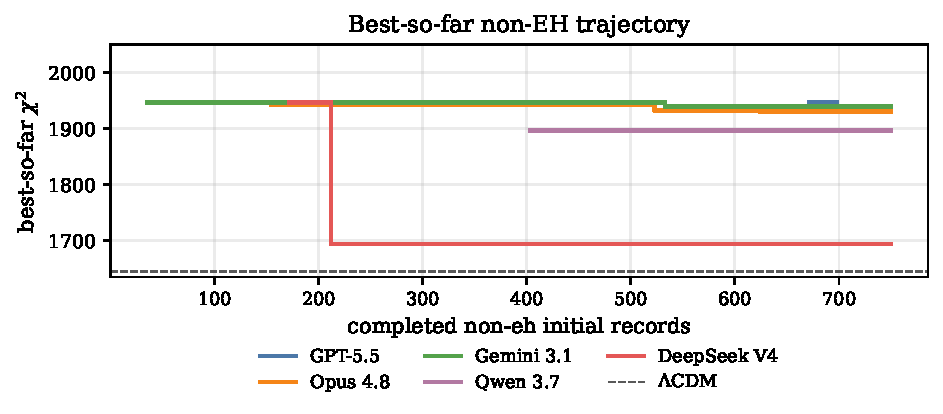
\includegraphics[width=0.88\textwidth]{figures/best_so_far_non_eh.pdf}
\caption{Best-so-far non-EH value as a function of completed non-EH initial records, plotted only after the best-so-far value enters the $\chi^2<2000$ display range.  The dashed reference line is the fixed $\Lambda$CDM value, not the non-EH refinement threshold.}
\label{fig:best-so-far-noneh}
\end{figure*}

The contrast between open search and non-EH search is the main physics message of the benchmark.  All agents can locate a good EH-anchored expansion history, but only a subset repeatedly finds non-EH backgrounds below $\chi^2=2000$.  Even the best such background remains worse than $\Lambda$CDM by roughly 48.6 in $\chi^2$ and worse than the best open-search branch by roughly 55.9.  Thus the non-EH candidates are interesting as discovered runnable structures, not as competitive replacements for the EH-anchored basin on DES-SN plus DESI-DR2 BAO background data.

\subsection{Agent-level behavior}
\label{subsec:agent-comparison}

\begin{figure}[t]
\centering
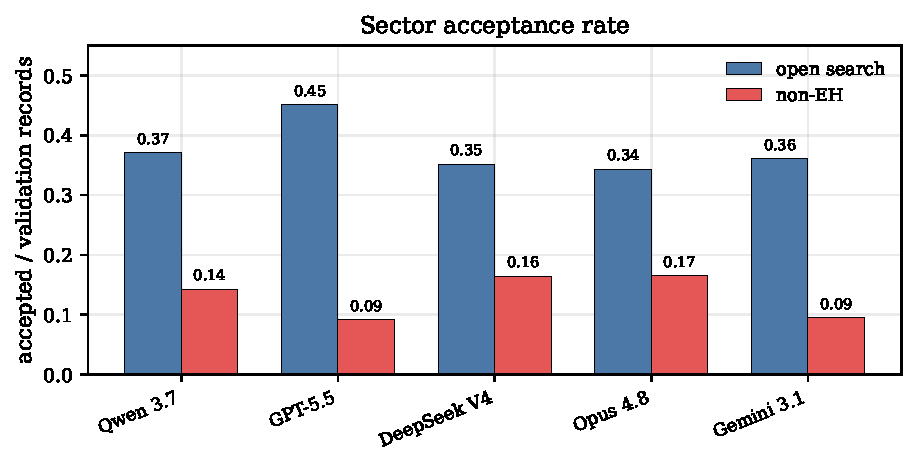
\includegraphics[width=0.48\textwidth]{figures/sector_acceptance.pdf}
\caption{Accepted fraction by sector.  Acceptance is a robustness diagnostic: it measures how often an agent reaches a Solver-evaluable background, not whether the resulting background has a low $\chi^2$.}
\label{fig:sector-acceptance}
\end{figure}

\begin{figure}[t]
\centering
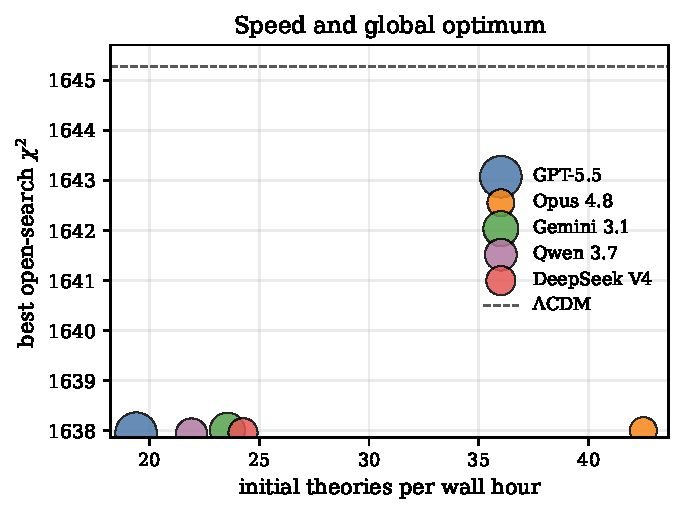
\includegraphics[width=0.48\textwidth]{figures/speed_quality_tradeoff.pdf}
\caption{Speed and global optimum.  The horizontal axis gives initial theories per wall hour; the vertical axis gives the best open-search $\chi^2$.  GPT-5.5 is shown as a censored run because it reached the wall-time limit before recording all 1500 initial theories.}
\label{fig:speed-quality}
\end{figure}

The five agents separate along different axes.  Qwen gives the best open-search minimum in the unified data set.  DeepSeek gives the strongest non-EH discovery and the largest number of non-EH hits below 2000.  GPT-5.5 gives a very stable open-search basin, with a low median and many hits below 1650, but its non-EH performance is weak and the job was wall-time censored.  Claude has the highest non-EH acceptance rate among the three new 1500-target agents, but its open-search accepted median is poor.  Gemini is balanced: it reaches a competitive open-search optimum and finds a non-EH branch below 2000, though it does not match DeepSeek's non-EH discovery.

\section{Validation Boundaries and Physical Interpretation}
\label{sec:validation-boundaries}

The validation performed here is a background-level filter, not a complete proof of covariant viability.  The symbolic stage removes independent higher-time derivatives in the homogeneous FLRW equations and the Solver enforces regular integration, the modified Friedmann constraint, and the data likelihood.  A fully viable theory must still pass perturbation-level tests: after solving nondynamical constraints, the scalar and tensor quadratic actions must have positive kinetic eigenvalues, acceptable sound speeds, no rapid gradient instabilities, and a regular constraint structure.  The present DES-SN plus DESI-DR2 BAO likelihood also does not include structure growth, weak lensing, redshift-space distortions, gravitational-wave propagation, or local-gravity screening.

The EFT interpretation is likewise diagnostic rather than automatic.  The trajectory-level cut controls $|H|/\Lambda$, but broad coefficient and scalar priors can still produce branches whose fitted corrections are large compared with the EH term.  Accepted operator lists also need not be inequivalent covariant theories: integration by parts, field redefinitions, curvature identities, and FLRW degeneracies can map different raw operator lists to the same background equations.  The results should therefore be read as best-per-family background representatives, pending a full operator-basis and perturbation audit.

\section{Discussion and Conclusions}
\label{sec:conclusion}

The unified benchmark shows that autonomous proposal agents can reliably recover high-quality EH-anchored dark-energy backgrounds under a deterministic modified-gravity validation pipeline.  The best open-search backgrounds improve the fixed $\Lambda$CDM reference by $\Delta\chi^2\simeq7.2$--$7.35$, and the differences among the best agents are small compared with the gap between open search and the non-EH sector.

The non-EH results are more discriminating.  DeepSeek's $\chiT=1693.860$ branch is the most interesting new-physics candidate found in these data: it is substantially better than the recurring $\chiT\simeq1946.87$ plateau and is structurally simple.  Nevertheless, it is still worse than the $\Lambda$CDM reference and much worse than the EH-anchored basin.  The current background data and priors therefore favor EH-anchored scalar histories, while non-EH backgrounds remain useful diagnostic targets for further search.

At the agent level, no single metric captures performance.  The relevant axes are global optimum, new-physics discovery, speed/efficiency, robustness/stability, and acceptance rate.  For future production searches, a practical strategy is to use a strong global optimizer for EH-anchored basins and a separate explorer tuned for the non-EH sector.  Follow-up work should add perturbation-level stability, growth and lensing likelihoods, gravitational-wave propagation constraints, local-gravity screening checks, and an operator-basis audit that removes FLRW-equivalent representatives.

\appendix
\section{Representative Accepted Theories}
\label{app:representatives}

This appendix lists compact coefficient-substituted representatives for the best open-search and non-EH families used in the unified benchmark.  Coefficients whose recovered value is exactly zero are omitted.  For GPT-5.5, Claude Opus 4.8, and Gemini 3.1 Pro the coefficients are read from the pulled Solver CSV files.  For Qwen and DeepSeek, which are taken from the earlier truncated 2000-run artifacts, the exact per-task Solver CSV files were not pulled; when necessary we use the recovered current-loop parameter memory and mark this explicitly.

We use the abbreviations
\begin{align}
{\cal R}_{3a}&=R^{cd}{}_{ab}R^{afh}{}_cR^b{}_{fdh},&
{\cal R}_{3b}&=R^{bd}{}_{ac}R^{agh}{}_bR^c{}_{dgh},\\
{\cal R}_{3c}&=R^b{}_aR^{cd}R^a{}_{cbd},&
{\cal R}_{3d}&=R_{ab}R^{adef}R^b{}_{def} .
\end{align}

\subsection{Open-search representatives}

\paragraph*{Qwen 3.7 1.} Scheduler id task\_000847\_expanded\_slot\_01\_lag\_1, scalar family phi1\_only, $\chiT=1637.930$. The coefficient vector is the nearest recovered joint-prior vector; its stored sample has $\chi^2=1637.930$.
\begin{widetext}
\begin{equation}
\mathscr{L}_{qwen,open,1}=\sqrt{-g}\left\{\Mp^2\left[\alpha R + \beta \Lambda^{-3} \phi_1 R^{bcd}_{a} R^{a}_{bcd} + \gamma \Lambda^{-4} \phi_1 \phi_1 R^{bcd}_{a} R^{a}_{bcd}\right] - \frac12(\nabla\phi_1)^2 - m_1^2f_1^2\left[1-\cos(\phi_1/f_1)\right]\right\}.
\end{equation}
\end{widetext}
\noindent Nonzero recovered coefficients: $\alpha=0.5,\; \beta=-4.67\times 10^{13},\; \gamma=9.69\times 10^{14}$. Representative operator content: $R; \phi_1 R^{bcd}_{a} R^{a}_{bcd}; \phi_1 \phi_1 R^{bcd}_{a} R^{a}_{bcd}$.

\paragraph*{GPT-5.5 2.} Scheduler id task\_000347\_expanded\_refine\_slot\_05\_lag\_1, scalar family phi1\_only, $\chiT=1637.953$.
\begin{widetext}
\begin{equation}
\mathscr{L}_{openai,open,2}=\sqrt{-g}\left\{\Mp^2\left[\alpha R + \beta \Lambda^{-2} R^2 + \gamma \Lambda^{-3} \phi_1 R R\right] - \frac12(\nabla\phi_1)^2 - \frac12m_1^2\phi_1^2\right\}.
\end{equation}
\end{widetext}
\noindent Nonzero recovered coefficients: $\alpha=0.5,\; \beta=1.4\times 10^{13},\; \gamma=-443.3$. Representative operator content: $R; R^2; \phi_1 R R$.

\paragraph*{DeepSeek V4 3.} Scheduler id task\_001266\_slot\_03\_lag\_1, scalar family phi1\_only, $\chiT=1637.962$. The coefficient vector is the nearest recovered joint-prior vector; its stored sample has $\chi^2=1637.962$.
\begin{widetext}
\begin{equation}
\mathscr{L}_{deepseek,open,3}=\sqrt{-g}\left\{\Mp^2\left[\alpha R + \beta \Lambda^{-2} R_{\mu\nu}R^{\mu\nu} + \gamma \Lambda^{-4} \phi_1 \phi_1 R^{ab} R_{ab}\right] - \frac12(\nabla\phi_1)^2 - m_1^2f_1^2\left[1-\cos(\phi_1/f_1)\right]\right\}.
\end{equation}
\end{widetext}
\noindent Nonzero recovered coefficients: $\alpha=0.5,\; \beta=-9134,\; \gamma=-7.01\times 10^{8}$. Representative operator content: $R; R_{\mu\nu}R^{\mu\nu}; \phi_1 \phi_1 R^{ab} R_{ab}$.

\paragraph*{Opus 4.8 4.} Scheduler id task\_001106\_slot\_04\_lag\_1, scalar family phi1\_only, $\chiT=1638.004$.
\begin{widetext}
\begin{equation}
\mathscr{L}_{claude,open,4}=\sqrt{-g}\left\{\Mp^2\left[\alpha R\right] - \frac12(\nabla\phi_1)^2 - m_1^2f_1^2\left[1-\cos(\phi_1/f_1)\right]\right\}.
\end{equation}
\end{widetext}
\noindent Nonzero recovered coefficients: $\alpha=0.5$. Representative operator content: $R$.

\paragraph*{Gemini 3.1 5.} Scheduler id task\_000281\_slot\_03\_lag\_1, scalar family both, $\chiT=1638.012$.
\begin{widetext}
\begin{equation}
\mathscr{L}_{gemini,open,5}=\sqrt{-g}\left\{\Mp^2\left[\alpha R\right] - \frac12(\nabla\phi_1)^2 - \frac12m_1^2\phi_1^2 - \frac12(\nabla\phi_2)^2 - m_2^2f_2^2\left[1-\cos(\phi_2/f_2)\right]\right\}.
\end{equation}
\end{widetext}
\noindent Nonzero recovered coefficients: $\alpha=0.5$. Representative operator content: $R$.

\subsection{Non-EH representatives}

\paragraph*{DeepSeek V4 1.} Scheduler id task\_000425\_expanded\_refine\_slot\_08\_lag\_1, scalar family both, $\chiT=1693.860$. The coefficient vector is the nearest recovered joint-prior vector; its stored sample has $\chi^2=1702.424$.
\begin{widetext}
\begin{equation}
\mathscr{L}_{deepseek,nonEH,1}=\sqrt{-g}\left\{\Mp^2\left[\alpha \Lambda^{-2} \phi_2 \phi_2 R\right] + \beta \Lambda^{-1} \phi_1 \Box\phi_1 \phi_2 + \gamma \Lambda^{-2} \phi_1 \Box\phi_1 \phi_2 \phi_2 - \frac12(\nabla\phi_1)^2 - m_1^2f_1^2\left[1-\cos(\phi_1/f_1)\right] - \frac12(\nabla\phi_2)^2 - \frac12m_2^2\phi_2^2\right\}.
\end{equation}
\end{widetext}
\noindent Nonzero recovered coefficients: $\alpha=-7251,\; \beta=-57.47,\; \gamma=3.64\times 10^{11}$. Representative operator content: $\phi_2 \phi_2 R; \phi_1 \Box\phi_1 \phi_2; \phi_1 \Box\phi_1 \phi_2 \phi_2$.

\paragraph*{Qwen 3.7 2.} Scheduler id task\_000809\_expanded\_refine\_slot\_03\_lag\_1, scalar family phi2\_only, $\chiT=1896.001$. The coefficient vector is the exact from pulled terminal summary; its stored sample has $\chi^2=1896.001$.
\begin{widetext}
\begin{equation}
\mathscr{L}_{qwen,nonEH,2}=\sqrt{-g}\left\{\Mp^2\left[\alpha \Lambda^{-2} \Box R + \beta \Lambda^{-4} {\cal R}_{3a} + \gamma \Lambda^{-2} \phi_2 \phi_2 R + \delta \Lambda^{-3} \phi_2 R^{ab} R_{ab} + \epsilon \Lambda^{-3} \phi_2 R^{bcd}_{a} R^{a}_{bcd} + \zeta \Lambda^{-4} \phi_2 \Box\phi_2 R\right] + \eta \phi_2 \Box\phi_2 + \theta \Lambda^{-2} \phi_2 \phi_2 \nabla^{a}\phi_2 \nabla_{a}\phi_2 - \frac12(\nabla\phi_2)^2 - \frac12m_2^2\phi_2^2\right\}.
\end{equation}
\end{widetext}
\noindent Nonzero recovered coefficients: $\alpha=4.11\times 10^{5},\; \beta=-3.51\times 10^{-6},\; \gamma=-8845,\; \delta=-0.03089,\; \epsilon=4.12\times 10^{7},\; \zeta=-6384,\; \eta=5.28\times 10^{15},\; \theta=1.42\times 10^{-10}$. Representative operator content: $\Box R; {\cal R}_{3a}; \phi_2 \phi_2 R; \phi_2 R^{ab} R_{ab}; \phi_2 R^{bcd}_{a} R^{a}_{bcd}; \phi_2 \Box\phi_2 R; \phi_2 \Box\phi_2; \phi_2 \phi_2 \nabla^{a}\phi_2 \nabla_{a}\phi_2$.

\paragraph*{Opus 4.8 3.} Scheduler id task\_001247\_expanded\_refine\_slot\_07\_lag\_1, scalar family phi2\_only, $\chiT=1930.880$.
\begin{widetext}
\begin{equation}
\mathscr{L}_{claude,nonEH,3}=\sqrt{-g}\left\{\Mp^2\left[\alpha \Lambda^{-2} R^2 + \beta \Lambda^{-2} R_{\mu\nu}R^{\mu\nu} + \gamma \Lambda^{-4} {\cal R}_{3c} + \delta \Lambda^{-4} {\cal R}_{3a} + \epsilon \Lambda^{-4} R\Box R + \zeta \Lambda^{-4} \phi_2 \phi_2 \phi_2 \phi_2 R + \eta \Lambda^{-4} \phi_2 \phi_2 R^{ab} R_{ab} + \theta \Lambda^{-4} \phi_2 \phi_2 R^{bcd}_{a} R^{a}_{bcd}\right] - \frac12(\nabla\phi_2)^2 - \frac12m_2^2\phi_2^2\right\}.
\end{equation}
\end{widetext}
\noindent Nonzero recovered coefficients: $\alpha=1.87\times 10^{-9},\; \beta=-1.09\times 10^{12},\; \gamma=1.9\times 10^{-10},\; \delta=-2.58\times 10^{11},\; \epsilon=-1.62\times 10^{15},\; \zeta=-170.1,\; \eta=4.54\times 10^{-5},\; \theta=6.11\times 10^{7}$. Representative operator content: $R^2; R_{\mu\nu}R^{\mu\nu}; {\cal R}_{3c}; {\cal R}_{3a}; R\Box R; \phi_2 \phi_2 \phi_2 \phi_2 R; \phi_2 \phi_2 R^{ab} R_{ab}; \phi_2 \phi_2 R^{bcd}_{a} R^{a}_{bcd}$.

\paragraph*{Gemini 3.1 4.} Scheduler id task\_001067\_expanded\_refine\_slot\_04\_lag\_1, scalar family phi2\_only, $\chiT=1939.014$.
\begin{widetext}
\begin{equation}
\mathscr{L}_{gemini,nonEH,4}=\sqrt{-g}\left\{\Mp^2\left[\alpha \Lambda^{-2} R_{\mu\nu\rho\sigma}R^{\mu\nu\rho\sigma} + \beta \Lambda^{-4} {\cal R}_{3b} + \gamma \Lambda^{-3} \phi_2 \phi_2 \phi_2 R + \delta \Lambda^{-3} \phi_2 R^{ab} R_{ab} + \epsilon \Lambda^{-4} \phi_2 \phi_2 R^{ab} R_{ab} + \zeta \Lambda^{-4} \phi_2 \phi_2 R^{bcd}_{a} R^{a}_{bcd}\right] + \eta \Lambda^{1} \Box\phi_2 + \theta \Lambda^{-2} \phi_2 \phi_2 \nabla^{a}\phi_2 \nabla_{a}\phi_2 - \frac12(\nabla\phi_2)^2 - \frac12m_2^2\phi_2^2\right\}.
\end{equation}
\end{widetext}
\noindent Nonzero recovered coefficients: $\alpha=-1.07\times 10^{4},\; \beta=-6\times 10^{-10},\; \gamma=3.47\times 10^{8},\; \delta=0.001309,\; \epsilon=-4.88\times 10^{14},\; \zeta=-4.48\times 10^{13},\; \eta=3.36\times 10^{-9},\; \theta=0.004467$. Representative operator content: $R_{\mu\nu\rho\sigma}R^{\mu\nu\rho\sigma}; {\cal R}_{3b}; \phi_2 \phi_2 \phi_2 R; \phi_2 R^{ab} R_{ab}; \phi_2 \phi_2 R^{ab} R_{ab}; \phi_2 \phi_2 R^{bcd}_{a} R^{a}_{bcd}; \Box\phi_2; \phi_2 \phi_2 \nabla^{a}\phi_2 \nabla_{a}\phi_2$.

\paragraph*{GPT-5.5 5.} Scheduler id task\_001346\_expanded\_slot\_04\_lag\_1, scalar family both, $\chiT=1946.871$.
\begin{widetext}
\begin{equation}
\mathscr{L}_{openai,nonEH,5}=\sqrt{-g}\left\{\Mp^2\left[\alpha \Lambda^{-4} \phi_2 \phi_2 R^{ab} R_{ab} + \beta \Lambda^{-4} \phi_2 \phi_2 R^{bcd}_{a} R^{a}_{bcd}\right] - \frac12(\nabla\phi_1)^2 - \frac12m_1^2\phi_1^2 - \frac12(\nabla\phi_2)^2 - \frac12m_2^2\phi_2^2\right\}.
\end{equation}
\end{widetext}
\noindent Nonzero recovered coefficients: $\alpha=-7699,\; \beta=2232$. Representative operator content: $\phi_2 \phi_2 R^{ab} R_{ab}; \phi_2 \phi_2 R^{bcd}_{a} R^{a}_{bcd}$.



\bibliographystyle{apsrev4-2}
\bibliography{main2}

\end{document}
